
\section{Método}

\begin{frame}{Exemplo de frases espaçadas tipo Afonso}
	\onslide<1,2,3,5>{\quad First Line of Text}
	\only<2,3>{\\ \quad \quad Second Line of Text}
	\onslide<3>{\\ \quad \quad \quad Third Line of Text}
\end{frame}

\begin{frame}{Rede de Petri Interpretada para Controle}
\begin{figure}[H]
  \centering
  \includegraphics[width=0.8\textwidth]{cipnExample/schemePresentation.tikz}
  \caption{Exemplo de sistema a ser controlado.}
  \label{fig:cipnexamplescheme}
\end{figure}
\end{frame}


\begin{frame}{Rede de Petri Interpretada para Controle}
\begin{figure}[H]
  \centering \includegraphics[width=\textwidth]{cipnExample/cipnPresentation.tikz}
  \caption{Exemplo de Rede de Petri interpretada para controle.}
  \label{fig:cipnexample}
\end{figure}
\end{frame}

\begin{frame}
  \begin{figure}[H]
    \centering
    \resizebox{0.7\textwidth}{!}{
   \includegraphics{cipnExample/cipnLadderPresentation.tikz}}
  \caption{Example of Control Interpreted Petri Net converted to Ladder.}
  \label{fig:cipnexampleLadder}
\end{figure}
\end{frame}

\begin{frame}{Datalog}
   \begin{figure}[ht]
       \begin{minipage}[b]{0.3\linewidth}
         \centering
 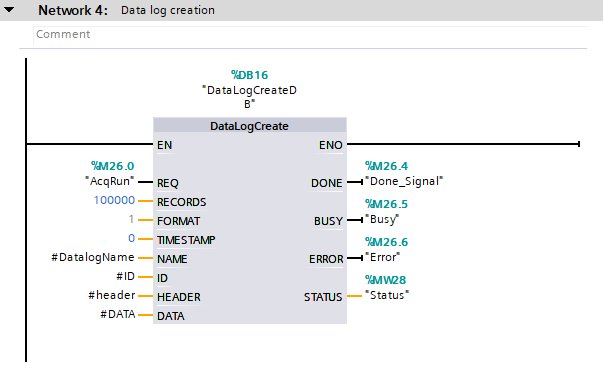
\includegraphics[width=\textwidth,clip,trim={0 0.8cm 3cm 0}]{tutorial/create}
       \end{minipage}
       \begin{minipage}[b]{0.3\linewidth}
         \centering
 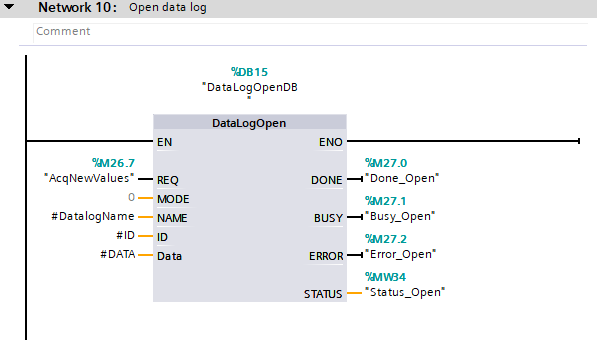
\includegraphics[width=\textwidth,clip,trim={0 0.4cm 3cm 0}]{tutorial/open}
\end{minipage}
       \begin{minipage}[b]{0.3\linewidth}
         \centering
	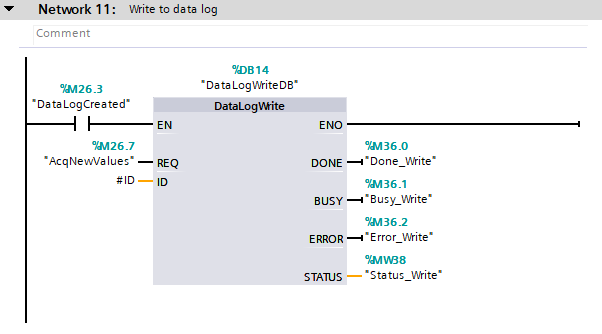
\includegraphics[width=\textwidth,clip,trim={0 0 3cm 0}]{tutorial/write}
       \end{minipage}
       \hspace{0.5cm}
       \begin{minipage}[b]{0.3\linewidth}
           \centering
	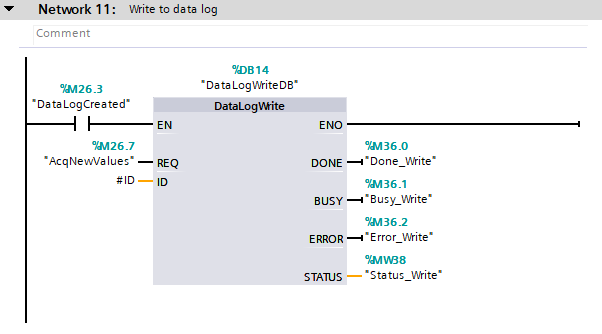
\includegraphics[width=\textwidth,clip,trim={0 1cm 3cm 0}]{tutorial/write}
       \end{minipage}
       \begin{minipage}[b]{0.3\linewidth}
           \centering
           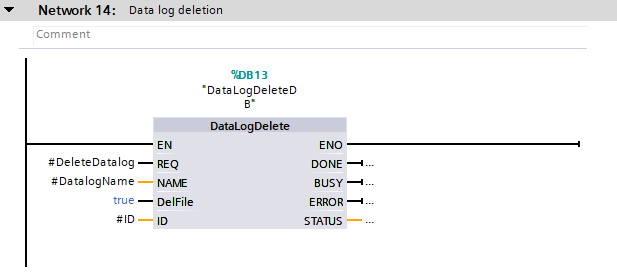
\includegraphics[width=\textwidth,clip,trim={0 -0.8cm 3cm 0}]{tutorial/delete}
       \end{minipage}
  \caption{Módulos da Planta.}
   \end{figure}
\end{frame}

%%% Local Variables:
%%% mode: latex
%%% TeX-master: "../presentation"
%%% End: